\RequirePackage{fix-cm}

\documentclass{svjour3}\usepackage[]{graphicx}\usepackage[]{color}
%% maxwidth is the original width if it is less than linewidth
%% otherwise use linewidth (to make sure the graphics do not exceed the margin)
\makeatletter
\def\maxwidth{ %
  \ifdim\Gin@nat@width>\linewidth
    \linewidth
  \else
    \Gin@nat@width
  \fi
}
\makeatother

\definecolor{fgcolor}{rgb}{0.345, 0.345, 0.345}
\newcommand{\hlnum}[1]{\textcolor[rgb]{0.686,0.059,0.569}{#1}}%
\newcommand{\hlstr}[1]{\textcolor[rgb]{0.192,0.494,0.8}{#1}}%
\newcommand{\hlcom}[1]{\textcolor[rgb]{0.678,0.584,0.686}{\textit{#1}}}%
\newcommand{\hlopt}[1]{\textcolor[rgb]{0,0,0}{#1}}%
\newcommand{\hlstd}[1]{\textcolor[rgb]{0.345,0.345,0.345}{#1}}%
\newcommand{\hlkwa}[1]{\textcolor[rgb]{0.161,0.373,0.58}{\textbf{#1}}}%
\newcommand{\hlkwb}[1]{\textcolor[rgb]{0.69,0.353,0.396}{#1}}%
\newcommand{\hlkwc}[1]{\textcolor[rgb]{0.333,0.667,0.333}{#1}}%
\newcommand{\hlkwd}[1]{\textcolor[rgb]{0.737,0.353,0.396}{\textbf{#1}}}%
\let\hlipl\hlkwb

\usepackage{framed}
\makeatletter
\newenvironment{kframe}{%
 \def\at@end@of@kframe{}%
 \ifinner\ifhmode%
  \def\at@end@of@kframe{\end{minipage}}%
  \begin{minipage}{\columnwidth}%
 \fi\fi%
 \def\FrameCommand##1{\hskip\@totalleftmargin \hskip-\fboxsep
 \colorbox{shadecolor}{##1}\hskip-\fboxsep
     % There is no \\@totalrightmargin, so:
     \hskip-\linewidth \hskip-\@totalleftmargin \hskip\columnwidth}%
 \MakeFramed {\advance\hsize-\width
   \@totalleftmargin\z@ \linewidth\hsize
   \@setminipage}}%
 {\par\unskip\endMakeFramed%
 \at@end@of@kframe}
\makeatother

\definecolor{shadecolor}{rgb}{.97, .97, .97}
\definecolor{messagecolor}{rgb}{0, 0, 0}
\definecolor{warningcolor}{rgb}{1, 0, 1}
\definecolor{errorcolor}{rgb}{1, 0, 0}
\newenvironment{knitrout}{}{} % an empty environment to be redefined in TeX

\usepackage{alltt}                     % onecolumn (standard format)
%\documentclass[smallcondensed]{svjour3}     % onecolumn (ditto)
%\documentclass[smallextended]{svjour3}       % onecolumn (second format)
%\documentclass[twocolumn]{svjour3}          % twocolumn
%

\usepackage{graphicx}
\usepackage{mathptmx}      
\usepackage{amsmath}
\usepackage{graphicx}
\usepackage{booktabs}
\usepackage{multirow}
\usepackage{cite}
\usepackage{caption}
\usepackage{natbib}


\journalname{Sankhya B}
\IfFileExists{upquote.sty}{\usepackage{upquote}}{}
\begin{document}
%\SweaveOpts{concordance=TRUE}

\title{Comparing Different Planned Missingness Designs in Longitudinal Studies}

\author{Josephine Wood \and Gregory J. Matthews \and Nicholas Illenberger \and Jennifer Pellowski \and Ofer Harel}

\institute{J. Wood \and G. J. Matthews
          \at Loyola University Chicago \\
          1032 W. Sheridan Rd.\\
          Chicago IL, 60660 USA\\
          Tel: (773)508-3558
          \and
          N. Illenberger \and O. Harel 
				\at University of Connecticut \\
						215 Glennbrook Rd. Unit 420\\
						Storrs CT, 06269-4120 USA
              Tel: (860)486-6989 \\
		      \email{ofer.harel@uconn.edu}  
					\and
					J. Pellowski
					\at International Health Institute\\ 
					Brown School of Public Health 
					\and J. Pellowski 
					\at Department of Psychiatry and Human Behavior\\
					The Warren Alpert Medical School of Brown University.  
}

\date{Received: date / Accepted: date}
% The correct dates will be entered by the editor


\maketitle


\begin{abstract}
Planned Missingness (PM) designs, in which researchers deliberately collect only partial data, have enjoyed a recent growth in popularity. Among other benefits these designs have been proven capable of reducing the study costs and alleviating participant burden. Past research has shown that Split Form PM designs can be effective in simplifying complex surveys while Wave Missingness PM designs act similarly for Longitudinal studies. However, less work has been done to inform how to implement PM structures into studies which incorporate elements of both survey and longitudinal designs. Specifically, in studies where a questionnaire is given to participants at multiple measurement occasions the best way to design missingness is still unclear. To address this deficiency, data in this hybrid format was simulated under both Split Form and Wave Missingness PM structures. Multiple Imputation techniques were applied to estimate a multilevel logistic model in each of the simulations. Estimated parameters were compared to the true values to see which PM design allowed us to best capture the true model. The results of this study indicate that, compared to the Split Form Design, the Wave Missingness design consistently performed less effectively in capturing the multilevel model. Thus, in the context of longitudinal surveys this study recommends the use of Split Form missingness designs, which performs well under a number of different conditions.

\keywords{Planned Missingness \and Split Form \and Multiform \and Wave Missingness \and Multiple Imputation \and Missing Data.}
\end{abstract}

\section{Introduction}
\label{intro}
Planned Missingness (PM) designs are a type of experimental design in which some of the data is predetermined to be missing. While it may seem counterproductive to deliberately omit data from the collection process, PM designs have been shown to reduce both participant burden \citep{graham2006planned, saris20048} and the costs of a study \citep{graham2001planned}. Moreover, PM designs can actually increase the quality of collected data by increasing the breadth of a study \citep{little2013planned} as well as decreasing the effects of assessment reactivity and rates of unplanned missingness \cite{harel2015designed}. We further note that while PM designs decrease the efficiency of estimators \citep{rhemtulla2016asymptotic}, decreasing the cost per participant may allow researchers to enroll more participants in a study, offsetting some of the efficiency loss. \par

There have been many different incarnations of the PM design, each crafted to best suit the study at hand. For example, PM designs have been used in the study of longitudinal growth curves \citep{graham2001planned, mcardle1997expanding}, business research \citep{shoemaker1973principles}, behavioral studies \citep{harel2015designed}, biostatistics \citep{andres2006partial, wacholder1994partial}, and educational assessments \citep{zeger1997efficient, sirotnik1977incidence}. This paper focuses on two of the simplest and most applicable PM designs; the Split Form design \citep{raghunathan1995split} and the Wave Missingness design \citep{little2013planned}. While this paper covers these designs in more detail later, broadly speaking, the Split Form design entails measuring fewer points on a single measurement occasion \citep{raghunathan1995split}. The Wave Missingness design, on the other hand, requires missing an entire measurement occasion within a longitudinal study \citep{graham2001planned}. 

The issue we concern ourselves with arises when a longitudinal study requires multiple items to be collected at each measurement occasion. When implementing a multi-level regression model in this situation, we investigate which planned missingess design is more efficient and accurate. Previous research indicates that for the estimation of correlated latent growth curve models use of the three-form PM design, a special case of Split Form designs \citep{raghunathan1995split}, resulted in low bias on parameter estimates or standard error and high efficiency when compared with wave missingness designs \citep{rhemtulla2014planned}. As our model of interest is a mixed effects model, however, we can not be sure that this result will hold. \par 

To answer our question we performed a simulation study from data obtained in longitudinal research on HIV medication adherence and alcohol-interactivity beliefs \citep{pellowski2016alcohol}. For the PM designs mentioned we simulated sample data and then used multiple imputation (MI) \citep{little2014statistical}  techniques to analyze the data. The PM methods were subsequently evaluated through the assessmemt of the average bias, percent bias, mean squared error, coverage rates, confidence interval length, and estimated fraction of missing information (FMI) \citep{little2014statistical} for parameter estimates in a multilevel model. To make the results generalizable, the experiment was repeated under multiple scenarios: increased sample size, low inter-survey correlation, and high time effect. \par

To delineate the remainder of this paper, in Section 2 we go into more depth on the two PM designs previously mentioned and then move into a discussion on the modern Multiple Imputation technique for dealing with missing data. Next, in Section 3 we briefly describe the dataset we worked with and our method of simulation before moving on to the results of our analyses in Section 4 and a discussion in the final section. \par


\section{Designs and Methods}
\label{sec:1}
\subsection{Split Form Design}
\label{sec:1.1}

Split Form missingness designs \citep{raghunathan1995split}, also  known as Multi-Form \citep{little2013planned} or Matrix Sampling designs \citep{thomas2006evaluation}, are very aptly named. Instead of giving participants one large survey, researchers create multiple forms, each containing a subset of the full survey's questions. A common form setup is the three-form design \citep{graham1996maximizing} in which the full survey is split into four blocks: X, A, B, and C. Each form of the survey includes the X block as well as two of the remaining blocks. This leaves the configurations seen in Table \ref{tab:table10}, where "1" indicates that the block is included and "0" indicates that it is excluded. Note that every block appears in at least one form. By designing the forms in this manner we are able to estimate the relationship between any chosen items regardless of their blocks. That is, if we want to estimate the relationship between an item in block A and another in C, there is a form that allows this. \par

We need to talk about the other type of split design that we used here which was that X of the 8 questions are randomly omitted on each day.  

% \begin{table}[h!]
% 	\centering
% 	\caption{The Three Form PM Design}
% 	\label{tab:table10}
% 	\setlength{\tabcolsep}{1cm}
% 	\begin{tabular}{c|cccc}
% 		\toprule
% 		& \multicolumn{4}{c}{Block} \\
% 		Form & X & A & B & C \\
% 		\midrule
% 		1 & 1 & 1 & 1 & 0 \\
% 		2 & 1 & 1 & 0 & 1 \\
% 		3 & 1 & 0 & 1 & 1 \\
% 		\bottomrule
% 	\end{tabular}
% \end{table}


























\begin{knitrout}
\definecolor{shadecolor}{rgb}{0.969, 0.969, 0.969}\color{fgcolor}\begin{figure}
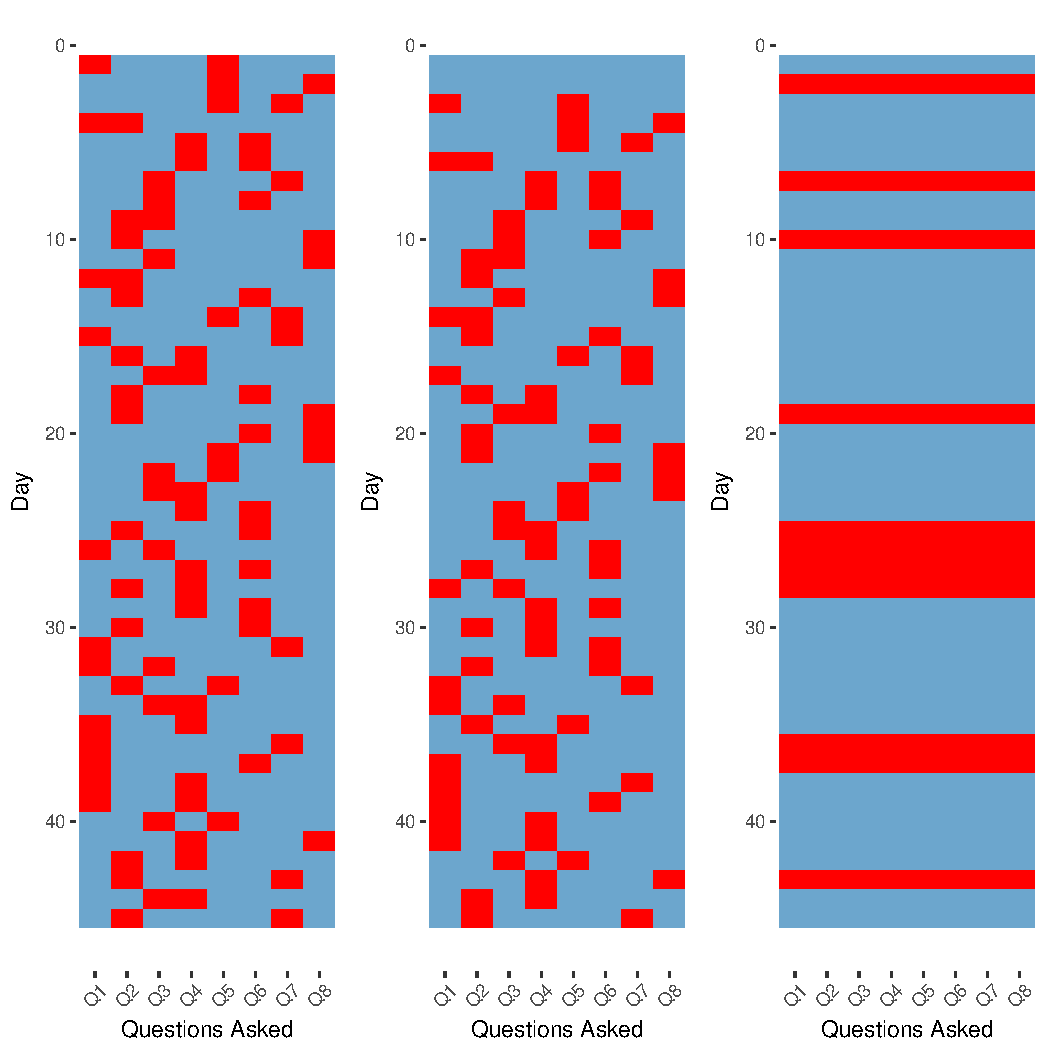
\includegraphics[width=\maxwidth]{figure/misslow-1} \caption[Low missingness]{Low missingness}\label{fig:misslow}
\end{figure}


\end{knitrout}

Figure \ref{fig:misslow} is 


An important consideration when designing a Split Form survey is question distribution. The X-block, being included in every form, should contain either the variables of greatest interest or those with the most predictive ability.
Placing central items in the X-block ensures they are always collected and minimizes the efficiency loss of our analyses \citep{thomas2006evaluation}. On the other hand, placing the most predictive variables in the X-block allows Multiple Imputation to more effectively impute missing values from the other blocks \citep{gottschall2012comparison}. Similarly, it is good practice to place variables which are predictive of each other in separate blocks \citep{gottschall2012comparison}. Note that when groupings are not as obvious, as in the previous example, pilot studies can help determine the predictive potential of variables. We may also wish to consider the cost and burden associated with an item when deciding which block to place it in. For example, if a critical item is overly expensive or difficult to obtain we may be better off excluding it from the X-block \citep{little2013planned}. \par

In additon, the number of blocks must be determined. Including more blocks in the design allows further increased missingness \citep{graham2006planned}. For example, consider two groups of researchers. The first group divides their survey into an X-block and three other blocks of equal size, each containing 25\% of the survey, and the second uses an X-block and nine others with 10\% of the items each. The researchers decide that a pair of blocks will be asked together in at least one of the forms to ensure efficient estimations. Based on this requirement, the first group can only reduce the length of their survey by 25\% while the second group can decrease the length of their survey by up to 70\%. \par

While increasing missingness may allow for further reductions in burden and cost, researchers must consider the disadvantages of more blocks. Inevitably, greater missingness leads to less efficient estimation \citep{rhemtulla2016asymptotic} but there is the added complication as more blocks introduce additional forms. If the second group of researchers in the example, for instance, decide that each form would contain the X-block and two of the other blocks, then they would be left with 36 total forms. For traditional paper surveys, this can make administering the survey difficult. However, for electronic questionaires, where form randomization can be automated, this is not an issue. Often, researchers using electronic surveys will give each participant a random sample of all survey items, in a way treating each item as its own block \citep{silvia2014planned}. Using this method, researchers reap the benefits of increased forms without the difficulty caused by manually building and administering these forms. \par

\subsection{Wave Missingness Design}
\label{sec:1.2}
While Split Form missingness can be applied to many experimental designs, the Wave Missingness design \citep{little2013planned} is unique to studies with multiple measurement occasions, or "waves". Unlike the Split Form design, where participants miss a subset of items in a single measurement occasion, the Wave Design entails randomizing participants to miss a measurement occasion entirely. An example of a Wave Missing design is shown in Table \ref{tab:table11} where data is collected monthly over the course of 5 months. However, each participant is only measured at three of these occasions. \par

\begin{table}[b!]
	\centering
	\caption{The Wave Missingness PM Design}
	\label{tab:table11}
	\setlength{\tabcolsep}{0.75cm}
	\begin{tabular}{c|ccccc}
		\toprule
		& \multicolumn{5}{c}{Month} \\
		Participant & 1 & 2 & 3 & 4 & 5 \\
		\midrule
		1 & 1 & 0 & 1 & 0 & 1 \\
		2 & 1 & 1 & 0 & 1 & 0 \\
		3 & 0 & 0 & 1 & 1 & 1 \\
		4 & 1 & 1 & 1 & 0 & 0 \\
		\bottomrule
	\end{tabular}
\end{table}

A relative advantage of the Wave Missingness design over the Split form design is increased control over the level of missingness. For studies with many measurement occasions, it is easy to make small changes to the amount of missing data. For example, the data described by \citet{pellowski2016alcohol} records measurements for 45 days. Missing eleven days here would result in 24.4\% missingness while missing twelve gives us 26.7\%. Further, Wave Missingness designs eclipse Split Form designs in terms of cost reduction \citep{little2013planned}. \par

Another advantage of this design is many longitudinal study designs already use the Wave Missingness structure \citep{little2013planned}. Cohort Sequential Designs require cohorts of different ages to be followed longitudinally in such a way that the information from one cohort can be used to impute values for another \citep{little2013longitudinal, duncan2013introduction}. For example, there were three cohorts of ages 10, 11, and 12 at baseline and measured annually for four years. Although measurement only occurs at four waves we can frame this as a six-wave study where the 10-year old cohort has missing values at waves five and six, the 11-year old cohort at waves one and six, and the 12-year old cohort at waves one and two. Because the 10-year old cohort is the only group observed at the first wave, the missing values for the other groups are imputed using this information. By continuing in this manner the data that was collected over a four year period is extended it to cover six years, accelerating the study. The setup of this type of study is demonstrated in Table \ref{tab:table12}, where "1" and "0" respectively indicate an included and excluded wave. \par

\begin{table}[t!]
	\centering
	\caption{Cohort Sequential Design}
	\label{tab:table12}
	\setlength{\tabcolsep}{0.5cm}
	\begin{tabular}{c|cccccc}
		\toprule
		& \multicolumn{6}{c}{Age} \\
		Participant & 10 & 11 & 12 & 13 & 14 & 15 \\
		\midrule
		1 & 1 & 1 & 1 & 1 & 0 & 0\\
		2 & 0 & 1 & 1 & 1 & 1 & 0\\
		3 & 0 & 0 & 1 & 1 & 1 & 1\\
		\bottomrule
	\end{tabular}
\end{table}

Developmental time-lag models \citep{mcardle1997expanding} also make use of the Wave Missingness structure. As shown in Table \ref{tab:table13}, researchers observe participants at only two measurement occasions, varying the length between occasions for each participant, and then treat this two-time-point data as multi-time-point data with missing values. Under this framework they impute these missing values and estimate growth curve models. Estimating this type of model would normally require measuring participants at many time points. However, under the Wave Missingness design this is accomplished with only two measurement occasions per participant. These designs exemplify how useful the Wave Missingness structure is in accelerating longitudinal studies. \par

\begin{table}[b!]
	\centering
	\caption{Developmental Time-Lag Setup}
	\label{tab:table13}
	\setlength{\tabcolsep}{0.75cm}
	\begin{tabular}{c|cccc}
		\toprule
		& \multicolumn{4}{c}{Wave} \\
		Participant & 1 & 2 & 3 & 4 \\
		\midrule
		1 & 1 & 1 & 0 & 0 \\
		2 & 1 & 0 & 1 & 0 \\
		3 & 1 & 0 & 0 & 1 \\
		\bottomrule
	\end{tabular}
\end{table}

\subsection{Multiple Imputation}
\label{sec:1.3}
\subsubsection{Missing Data Mechanisms}
\label{sec:1.3.1}
Before describing Multiple Imputation and how it can be applied to PM designs it is important to first understand how data become incomplete. Suppose we have a dataset, $Y_{com}$, with some missing values. We define the missingness, $R$, to be an indicator variable which equals 0 where $Y_{com}$ is observed and 1 where the corresponding value in $Y_{com}$ is missing. Missing data mechanisms describe the proposed probabilistic relationship between $R$ and the values in $Y_{com}$, observed or unobserved \citep{little2014statistical}. \par

The first missing data mechanism, missing at random (MAR), was defined by \citet{rubin1976inference}. Data are considered MAR when the missingness does not depend on unobserved values but may depend upon other observed variables. For instance, if men are less likely to report their incomes than women but the level of income itself does not affect the probability of reporting, then we can say the missingness govern income is MAR. \par

Later, \citet{little2014statistical} described two additional mechanisms which lead to missing values: missing completely at random (MCAR) and missing not at random (MNAR) \citep{little2014statistical}. The first, MCAR, is used to describe a situation in which the missingness is independent of the observed or unobserved data. That is, the missing values are simply a random subset of the full data. On the other hand, data is said to be MNAR when the missingness is related to the unobserved data; in a survey people may be less willing to provide their income if it is extremely high or low, for example. \par

If we have prior knowledge concerning the relationship between unobserved values, indicated by $R$, and the observed values, then Multiple Imputation can yield efficient estimates even under MNAR \citep{harel2007multiple}. However, because this is not typically the case, MI is most often implemented when data is MCAR or MAR \citep{little2014statistical}. \par

As a consequence of allowing researchers to decide which values in a dataset are observed and unobserved, PM designs grant control over the missing data mechanism. Because of this, MI is an appealing option for researchers utilizing a PM design. If implemented properly, data should conform to either the MCAR or MAR assumption. For instance, if medical researchers decide not to collect blood pressure on a completely random subset of patients there is no reason to believe the missing blood pressures differ significantly from the observed ones. This fact allows for the use of MI and other modern missing data techniques such as the Full Information Maximum Likelihood approach \citep{dempster1977maximum} \par

\subsubsection{The Multiple Imputation Procedure}
\label{sec:1.3.2}
Multiple Imputation is used to obtain statistically valid inferences in spite of missing data. MI works by replacing unobserved values with a set of plausible values in a way which allows us to account for uncertainty in the imputation process. Repeatedly using an imputation technique, every missing value in the incomplete dataset is replaced with a fixed number of imputed values. This process allows for the creation of multiple complete datasets, on which users can run complete-data procedures. If, for instance, we imputed $M$ possible values for every missing value we would obtain $M$ different completed datasets. Once created, the analysis of interest can be performed on each of them and, using rules defined by \citet{little2014statistical} and \citet{rubin2004multiple}, combine the results to obtain a single inference. \par

Suppose we are interested in estimating a certain parameter such as the mean of a variable or a regression coefficient. If $\theta$ is the parameter of interest, let $\widehat{\theta_1}, \widehat{\theta_2}, ... \widehat{\theta_M}$ be the estimates of $\theta$ and let $S_1, S_2, ... S_M$ be the corresponding estimated standard errors from the $M$ imputed datasets. We can aggregate these results using the combining rules specified by \citet{little2014statistical} and \citet{rubin2004multiple}. \par
The overall MI estimate of $\theta$ is defined as,

\begin{equation}
\widehat{\theta} = \sum_{n=1}^{M} \widehat{\theta_n}.
\end{equation}

From here we can compute the sample variance of this estimate by calculating the between-imputation component, $B_M = \sum_{n=1}^{M} (\widehat{\theta_n} - \widehat{\theta})^2 / (M-1)$, and the within-imputation component, $W_M = \sum_{n=1}^{M} S_n^2 / M$. These components are combined to obtain the overall sample variance of our MI estimate as follows:

\begin{equation}
T_M = W_M + (1+1/M)*B_M.
\end{equation}

These equations form the basis of Rubin's combining rules and provide unbiased parameter estimates accounting for the inherent uncertainty in the imputation process \citep{raghunathan2015missing}. For a more in depth explanation of these methods we refer readers to \citet{little2014statistical}. \par

When using Multiple Imputation, researchers must decide on the number of imputations, $M$, to use. Generally, as the level of missingness decreases the number of imputations needed does as well. If less than 20\% of the requisite data is missing, for instance, five or tien imputations will suffice \citep{raghunathan2015missing}. However, at its roots, MI is a simulation technique and thus, the greater $M$ is the more stable our estimates become \citep{harel2007inferences}. \citet{graham2007many} recommend that if computational power is not a limiting factor, then setting $M=100$ is good practice. \par

\section{Data and Simulations}
\label{sec:2}
\subsection{Data}
\label{sec:2.1}
The dataset the simulations are based on originated in a study by \citet{pellowski2016alcohol}. The data was collected in an attempt to determine the day-level relationship between alcohol use, its interactive toxicity beliefs, and adherence to antiretroviral therapy (ART) amongst patients with HIV. Previous studies note that alcohol use combined with the perception that mixing alcohol and ARTs can cause adverse effects, correlated with non-adherence to ARTs \citep{kalichman2009prevalence, kalichman2012alcohol}. However, \citet{pellowski2016alcohol} pointed out that past research collected data over extended periods of time, preventing the identification a day-level interaction. Unlike others, this study was able to determine whether alcohol use and missed medication doses occurred on the same day. \par

The study employed an observational cohort design, following sixty participants over forty-five consequtive days via a daily questionnaire. Questions in the survey concerned livelihood insecurities from the previous day as well as alcohol use. The analysis included eight particular questions: two binary questions on housing insecurity, four binary questions on food insecurity, and two questions concerning alcohol use (one binary variable and one count variable). The exact questions can be found in Table \ref{tab:table1}. \par

\begin{table}[t]
	\centering
	\caption{Survey Questions}
	\label{tab:table1}
	\begin{tabular}{cp{6.5cm}c}
		\toprule
		Item Number & Question & Responses\\
		\midrule
		1 & I worried about having a place to stay yesterday. & 1.Yes $\>$ 2.No \\
		2 & I could not get to where I needed to go yesterday. & 1.Yes $\>$ 2.No \\
		3 & I worried about my food running out yesterday. & 1.Yes $\>$ 2.No \\
		4 & I ate less than I needed to yesterday. & 1.Yes $\>$ 2.No \\
		5 & I was hungry, but did not eat because I couldn't afford food. & 1.Yes $\>$ 2.No \\
		6 & I got food from a pantry, church, agency, friend or the street yesterday. & 1.Yes $\>$ 2.No \\
		7 & Did you drink alcohol yesterday? & 1.Yes $\>$ 2.No \\
		8 & How many alcohol drinks did you have yesterday? & 0-20 \\
		\bottomrule
	\end{tabular}
\end{table}

Beyond the daily questionnaire, data was also collected through a computer-assisted interview on behavioral, psychosocial, and cognitive factors (ex. Income, alcohol-toxicity beliefs, education, etc.) which have been shown to be associated with medication adherence. These values were only collected at baseline and are considered time independent. The variables from this assessment used in our analysis concerned education level, income, age, beliefs about the interactivity of alcohol with ART medication, depression, and alcohol abuse. \par

\subsection{Simulations}
\label{sec:2.2}
The first step in the process of creating the simulated datasets was to obtain parameter estimates from \citet{pellowski2016alcohol} and to quantify the relationships between variables. These estimated relationships were treated as the "true" relationships and one thousand samples were drawn using these parameters. The purpose of simulating these datasets was to see how well they captured the true relationship between daily medication adherence on a certain day, whether or not a participant drank that day, and their beliefs about alcohol-medication interactivity (included as a Z-transformed test score). Specifically, our model of interest is the random intercept model with time effect found below: \\

\begin{align*}
logit(MissedDose) &= \beta_{0j} + \beta_1*DrinkYN + \beta_2*ZAlcTox +\beta_3*Day \\
Level 2: \beta_{0j} &= \gamma_0 + \epsilon_j
\end{align*}
where, \\ \\
$MissedDose = 1$ if the participant did not adhere to the ART, 0 otherwise. \\
$DrinkYN = 1$ if the participant drank on a given day, 0 otherwise.\\
$ZAlcTox =$ Z-transformed score on an alcohol-antiretroviral interactive toxicity scale developed by Kalichman \cite{kalichman2009prevalence}. \\
$Day =$ The number of days since the study began, 0-44. \\
$j =$ participant index, 1-60. \\
$\epsilon_j  \sim N(0, \sigma^2)$. \\ \\


Based on the observed data, the true values of the parameters, $\gamma_0, \beta_1, \beta_2$, $\beta_3$, and $\sigma^2$ were found to be -2.3, 0.56, 1.28, 0.2, and 1.0 respectively. \par
Once the samples were drawn, they were transformed under the three different missingness structures. These were the Split-Form and Wave Missingness designs previously mentioned as well as a variation on the Split-Form design where a few measurement occasions (here, two days per participant) are fully observed. To clarify this difference, see the hypothetical application of these designs to a five question multi-day survey in Table \ref{tab:table14}. As in the previous tables, "1" indicates an observed occasion while "0" indicates a missing one. We see that the Split Form design entails missing two items on each of the days. The altered Split Form, while similar, is fully measured on two of the measurement occasions. Because there are days which are fully observed, the relationships between variables may be clearer, allowing the imputation procedure to run more effectively. On the other hand, the Wave Missingness design shows two days in which no questions are asked but the full questionnaire is given on the remaining days. \par

\begin{table}[t!]
	\centering
	\caption{Different Planned Missingness Designs}
	\setlength{\tabcolsep}{0.45cm}
	\label{tab:table14}
	\hspace*{-1cm}
	\begin{tabular}{c|c|ccccc}
		\toprule
		Design & Day & Q1 & Q2 & Q3 & Q4 & Q5 \\
		\midrule
		\multirow{5}{*}{Split Form}
		& 1 & 1 & 1 & 0 & 0 & 1 \\
		& 2 & 0 & 0 & 1 & 1 & 1 \\
		& 3 & 0 & 1 & 1 & 0 & 1 \\
		& 4 & 1 & 0 & 1 & 1 & 0 \\
		& 5 & 1 & 1 & 0 & 1 & 1 \\
		\midrule
		\midrule
		\multirow{5}{*}{Altered Split Form}
		& 1 & 1 & 1 & 1 & 1 & 1 \\
		& 2 & 1 & 1 & 1 & 1 & 1 \\
		& 3 & 0 & 0 & 1 & 1 & 1 \\
		& 4 & 1 & 1 & 0 & 1 & 0 \\
		& 5 & 0 & 1 & 1 & 0 & 1 \\
		\midrule
		\midrule
		\multirow{5}{*}{Wave Missingness}
		& 1 & 1 & 1 & 1 & 1 & 1 \\
		& 2 & 0 & 0 & 0 & 0 & 0 \\
		& 3 & 1 & 1 & 1 & 1 & 1 \\
		& 4 & 1 & 1 & 1 & 1 & 1 \\
		& 5 & 0 & 0 & 0 & 0 & 0 \\
		\bottomrule
	\end{tabular}
	\hspace*{-1cm}	
\end{table}

Additionally, for each different Missingness pattern we imposed low, medium, and high levels of missingness roughly corresponding to 25\%, 50\%, and 75\% missing data. Previous work by \citet{rhemtulla2014planned} found that for low levels of missingness (25\%) the Three-Form design outperforms the Wave Missingness design in capturing latent growth curve model parameters. However, because only low-levels of missingness are tested it is unknown whether this relationship holds at moderate or high levels. We hope that by including these different levels of missingness we will be able to see how these designs perform at all levels of the missingness spectrum. \par
Once missingness was created, Multiple Imputation techniques were applied to estimate the relationship between medication adherence and the other variables in our model. Because we have control over the missing data mechanism, we know the data is MCAR. This fact allows for the principled use of MI techniques. Using the R package $\{$mice$\}$ \citep{mice2011imputation} our binary variables (Q1-Q7) were imputed using a logistic model based approach while the count variable (Q8) was imputed using predictive mean matching. \par

After imputating, a logistic random-intercept model was estimated for each of the imputed datasets and combined using Rubin's Rules \citep{rubin2004multiple}. From here, the results from each PM design were evaluated based on bias, percent bias, mean squared error (MSE), coverage, confidence interval (CI) length, and the fraction of missing information (FMI). The FMI is a measure of how much of the MI sample variance comes from differences between imputations. In addition to comparing the results between each of the PM designs, the same analyses were also performed before missingness was imposed. \par

When determining if the PM designs are performing sufficiently, it is important to consider how well the simulated samples performed before adding a missingness structure. For example, consider two full data samples with respective biases on the $\beta_1$ estimate of 0.13 and 0.15. Further, after imposing different PM design structures on these samples, the average biases are 0.14 and 0.15 respectively. It would be unfair to claim that the first PM design performed better than the second because, by chance, it was based off of a more representative sample. This fact was considered when determining the evaluation criteria. \par

For bias, percent bias, and MSE we claimed that an increase of more than 40\% in these measurements after imposing missingness indicates that the PM design is inappropriate. For instance, if the complete data shows a percent bias of 10\%, anything higher than 14\% would be unacceptable. An increase of this size has the ability to negatively effect efficiency of our estimation. Based on the work of \citet{collins2001comparison} we also regard coverages of less than 90\% as unacceptable. If a 95\% CI has a true coverage of 90\% than the Type I error rate is double what it should be. Because MI accounts for uncertainty in the imputation process, coverages should be similar despite the added missingness. In terms of confidence interval lengths, if one PM design provides similar rates of coverage to another while maintaining shorter intervals than this is considered the better of the two methods. For equal coverage rates, shorter intervals imply more power. The FMI, which quantifies the uncertainty in our imputation process, is simply reported for each PM design. While less uncertainty in the imputations can be beneficial, less variation does not necessarily imply accuracy. Thus, FMI should be taken in the context of the other measurements. \par

This process was repeated under the three modified simulation scenarios mentioned in the following sections. Note that while typically these PM designs would be compared against the results obtained using a complete case analysis \citep{rhemtulla2016asymptotic}, this approach was avoided as it would fundamentally alter the form of the data. Specifically, complete case analysis removes any observation with any missing values. Then, for the Split Form design this would remove all observations. In the Wave Missingness setup, complete case analysis would shorten the length of the longitudinal study. If a participant was missing values on 11 of the 45 days, then complete case analysis would have made the data resemble a longitudinal study held over 34 days. Hence, this comparison is invalid. \par

\subsubsection{Increased Sample Size}
In order to evaluate the impact of sample size on estimation, the original sample size of 60 participants was expanded to 120. The rest of the simulation process was carried out as before. As noted earlier, the cost savings gleaned from the PM designs could allow us to enroll more participants. Thus, even if one design performed more optimally than the others, if all designs also perform acceptably well at high samples, researchers can design missingness in whichever method is most convenient. Furthermore, because Wave Missingness allows for greater savings, an increase in sample size is more reasonable for that type of missingness. \par
\subsubsection{Low Inter-Survey Correlation}
For our second simulation scenario we looked to determine the effect of decreased inter-survey correlation on which PM design would perform best. To clarify, consider the fact that answers given on a particular day may be correlated with one another- the two questions on housing insecurity, for example, are likely to be "yes" on the same days. While this fact was accounted for in the original simulations, it was not in this set of simulations. If the probability of answering "yes" on Question 2, for instance, was a function of the answer to Question 1 and the baseline variables in the original simulations, then in this scenario it is a function of only the baseline variables. This implies that each of the questions are conditionally independent of each other given the baseline variables. If researchers have a questionnaire where they do not expect any of the answers to be obviously related the results here may help to choose which missingness design would be most optimal. \par
\subsubsection{High Time Effect}
In the final scenario, the goal was to determine which PM design would lead to the best estimates when time has a disproportionately large effect on our outcome variable. To do this we changed the value of the parameters $\gamma_0, \beta_1, \beta_2,$ and $\beta_3$ to -4.6, 0.28, 0.64, and 0.2 respectively. Note that instead of increasing the value of $\beta_3$, the slope for time effect, all the other parameters were decreased. This was done because $\beta_3$ was already fairly large and increasing its value further would cause the probability of missing a dose to rapidly approach 1. Decreasing the other variables effects ensured that time has a disproportionate effect without this problem. The results of this section may prove useful to researchers who believe that the overall passage of time plays a larger role in their outcome than a measurement taken at one specific point. \par

\section{Results}
\label{sec:3}
\subsection{Primary Simulation}
\label{sec:3.1}
The first set of simulations run contained the parameters in the random-intercept logistic model with $\gamma_0 = -2.3$, $\beta_1 = 0.56$, $\beta_2 = 1.28$, and $\beta_3 = 0.2$. The effects of the variables here are comparable to those found in the original dataset. This fact implies that we can interpret the results here to show what may have occurred if the original study had implemented a PM design. Before we imposed a missingness structure on the 1,000 simulated samples we obtained the full data results shown in Table \ref{tab:table2}. Note that the full data results for the other simulation scenarios are also provided in this table for ease of reference.

\begin{knitrout}
\definecolor{shadecolor}{rgb}{0.969, 0.969, 0.969}\color{fgcolor}
\begin{tabular}{l|l|l|r|r|r|r|r|r}
\hline
Design & Missingness & Parameter & Bias & Pct Bias & MSE & Coverage & CI Length & FMI\\
\hline
 &  & $\gamma_0$ & 0.042 & -1.817 & 0.018 & 0.988 & 0.702 & 0.002\\
\cline{3-9}
 &  & $\beta_1$ & -0.071 & -25.122 & 0.269 & 0.983 & 2.534 & 0.236\\
\cline{3-9}
 &  & $\beta_2$ & 0.008 & 1.253 & 0.024 & 0.932 & 0.585 & 0.000\\
\cline{3-9}
 & \multirow{-4}{*}{\raggedright\arraybackslash Low} & $\beta_3$ & 0.000 & -0.886 & 0.000 & 0.944 & 0.017 & 0.001\\
\cline{2-9}
 &  & $\gamma_0$ & 0.039 & -1.684 & 0.018 & 0.990 & 0.709 & 0.011\\
\cline{3-9}
 &  & $\beta_1$ & -0.102 & -36.186 & 0.271 & 0.998 & 3.500 & 0.534\\
\cline{3-9}
 &  & $\beta_2$ & 0.008 & 1.207 & 0.024 & 0.933 & 0.586 & 0.002\\
\cline{3-9}
 & \multirow{-4}{*}{\raggedright\arraybackslash Medium} & $\beta_3$ & 0.000 & -0.419 & 0.000 & 0.946 & 0.017 & 0.007\\
\cline{2-9}
 &  & $\gamma_0$ & 0.028 & -1.242 & 0.027 & 0.985 & 0.791 & 0.030\\
\cline{3-9}
 &  & $\beta_1$ & -0.107 & -38.054 & 0.418 & 0.988 & 4.268 & 0.630\\
\cline{3-9}
 &  & $\beta_2$ & 0.012 & 1.869 & 0.027 & 0.932 & 0.613 & 0.005\\
\cline{3-9}
\multirow{-12}{*}{\raggedright\arraybackslash Split Form} & \multirow{-4}{*}{\raggedright\arraybackslash High} & $\beta_3$ & 0.000 & -0.471 & 0.000 & 0.946 & 0.020 & 0.020\\
\cline{1-9}
 &  & $\gamma_0$ & 0.042 & -1.832 & 0.018 & 0.990 & 0.701 & 0.001\\
\cline{3-9}
 &  & $\beta_1$ & -0.069 & -24.401 & 0.283 & 0.983 & 2.508 & 0.218\\
\cline{3-9}
 &  & $\beta_2$ & 0.008 & 1.272 & 0.024 & 0.933 & 0.585 & 0.000\\
\cline{3-9}
 & \multirow{-4}{*}{\raggedright\arraybackslash Low} & $\beta_3$ & 0.000 & -0.949 & 0.000 & 0.944 & 0.017 & 0.001\\
\cline{2-9}
 &  & $\gamma_0$ & 0.040 & -1.760 & 0.018 & 0.988 & 0.704 & 0.007\\
\cline{3-9}
 &  & $\beta_1$ & -0.117 & -41.573 & 0.277 & 0.990 & 3.385 & 0.508\\
\cline{3-9}
 &  & $\beta_2$ & 0.008 & 1.286 & 0.024 & 0.931 & 0.585 & 0.002\\
\cline{3-9}
 & \multirow{-4}{*}{\raggedright\arraybackslash Medium} & $\beta_3$ & 0.000 & -0.986 & 0.000 & 0.945 & 0.017 & 0.005\\
\cline{2-9}
 &  & $\gamma_0$ & 0.036 & -1.592 & 0.021 & 0.989 & 0.742 & 0.022\\
\cline{3-9}
 &  & $\beta_1$ & -0.158 & -56.111 & 0.394 & 0.992 & 4.336 & 0.662\\
\cline{3-9}
 &  & $\beta_2$ & 0.012 & 1.809 & 0.026 & 0.934 & 0.601 & 0.006\\
\cline{3-9}
\multirow{-12}{*}{\raggedright\arraybackslash Altered Split Form} & \multirow{-4}{*}{\raggedright\arraybackslash High} & $\beta_3$ & 0.000 & -1.487 & 0.000 & 0.941 & 0.018 & 0.021\\
\cline{1-9}
 &  & $\gamma_0$ & 0.040 & -1.765 & 0.018 & 0.988 & 0.703 & 0.005\\
\cline{3-9}
 &  & $\beta_1$ & -0.094 & -33.425 & 0.238 & 0.993 & 2.995 & 0.433\\
\cline{3-9}
 &  & $\beta_2$ & 0.008 & 1.251 & 0.024 & 0.934 & 0.585 & 0.001\\
\cline{3-9}
 & \multirow{-4}{*}{\raggedright\arraybackslash Low} & $\beta_3$ & 0.000 & -0.875 & 0.000 & 0.943 & 0.017 & 0.002\\
\cline{2-9}
 &  & $\gamma_0$ & 0.028 & -1.223 & 0.018 & 0.995 & 0.744 & 0.051\\
\cline{3-9}
 &  & $\beta_1$ & -0.088 & -31.121 & 0.240 & 0.992 & 3.497 & 0.718\\
\cline{3-9}
 &  & $\beta_2$ & 0.009 & 1.436 & 0.024 & 0.933 & 0.588 & 0.006\\
\cline{3-9}
 & \multirow{-4}{*}{\raggedright\arraybackslash Medium} & $\beta_3$ & 0.000 & -1.326 & 0.000 & 0.946 & 0.017 & 0.025\\
\cline{2-9}
 &  & $\gamma_0$ & -0.004 & 0.194 & 0.020 & 0.995 & 0.962 & 0.224\\
\cline{3-9}
 &  & $\beta_1$ & -0.080 & -28.263 & 0.234 & 0.985 & 3.791 & 0.886\\
\cline{3-9}
 &  & $\beta_2$ & 0.011 & 1.700 & 0.024 & 0.938 & 0.607 & 0.032\\
\cline{3-9}
\multirow{-12}{*}{\raggedright\arraybackslash Wave Missingness} & \multirow{-4}{*}{\raggedright\arraybackslash High} & $\beta_3$ & 0.000 & -3.304 & 0.000 & 0.970 & 0.020 & 0.148\\
\hline
\end{tabular}

\begin{kframe}

{\ttfamily\noindent\bfseries\color{errorcolor}{\#\# Error in column\_spec(1, width = "{}30em"{}): argument "{}column"{} is missing, with no default}}\begin{verbatim}
## % latex table generated in R 3.4.1 by xtable 1.8-2 package
## % Thu May 17 15:47:48 2018
## \begin{table}[ht]
## \centering
## \begin{tabular}{lllrrrrrr}
##   \hline
## "" & "" & "" & Coverage & Bias & MSE & FMI & CI Length & Pct Bias \\ 
##   \hline
##  &  &  & 0.968 & -0.023 & 0.120 & 0.018 & 1.414 & 0.498 \\ 
##    &  &  & 0.973 & 0.604 & 0.669 & 0.271 & 4.812 & 429.053 \\ 
##    &  &  & 0.955 & 0.010 & 0.048 & 0.003 & 0.827 & 3.263 \\ 
##    &  &  & 0.945 & -0.000 & 0.000 & 0.004 & 0.039 & -2.671 \\ 
##    &  &  & 0.972 & -0.048 & 0.128 & 0.059 & 1.506 & 1.060 \\ 
##    &  &  & 0.988 & 0.724 & 0.898 & 0.499 & 5.933 & 513.940 \\ 
##    &  &  & 0.958 & 0.025 & 0.047 & 0.013 & 0.834 & 7.927 \\ 
##    &  &  & 0.938 & -0.000 & 0.000 & 0.017 & 0.039 & -2.867 \\ 
##    &  &  & 0.984 & -0.178 & 0.370 & 0.132 & 2.050 & 3.882 \\ 
##    &  &  & 0.955 & 0.997 & 1.573 & 0.610 & 6.822 & 708.287 \\ 
##    &  &  & 0.965 & 0.044 & 0.060 & 0.036 & 0.966 & 13.650 \\ 
##    &  &  & 0.955 & -0.000 & 0.000 & 0.060 & 0.048 & -0.787 \\ 
##    &  &  & 0.966 & -0.019 & 0.119 & 0.011 & 1.401 & 0.415 \\ 
##    &  &  & 0.966 & 0.603 & 0.638 & 0.239 & 4.616 & 428.601 \\ 
##    &  &  & 0.956 & 0.014 & 0.048 & 0.002 & 0.827 & 4.254 \\ 
##    &  &  & 0.944 & -0.000 & 0.000 & 0.003 & 0.039 & -3.004 \\ 
##    &  &  & 0.978 & -0.045 & 0.124 & 0.053 & 1.493 & 0.988 \\ 
##    &  &  & 0.974 & 0.728 & 0.879 & 0.504 & 5.976 & 517.389 \\ 
##    &  &  & 0.954 & 0.024 & 0.051 & 0.011 & 0.838 & 7.437 \\ 
##    &  &  & 0.946 & -0.001 & 0.000 & 0.018 & 0.039 & -4.550 \\ 
##    &  &  & 0.984 & -0.117 & 0.196 & 0.112 & 1.759 & 2.557 \\ 
##    &  &  & 0.968 & 0.876 & 1.305 & 0.650 & 6.913 & 622.327 \\ 
##    &  &  & 0.963 & 0.026 & 0.051 & 0.034 & 0.892 & 8.265 \\ 
##    &  &  & 0.949 & -0.001 & 0.000 & 0.055 & 0.043 & -5.340 \\ 
##    &  &  & 0.968 & -0.057 & 0.127 & 0.038 & 1.454 & 1.249 \\ 
##    &  &  & 0.974 & 0.853 & 1.003 & 0.510 & 5.629 & 606.148 \\ 
##    &  &  & 0.959 & 0.006 & 0.046 & 0.006 & 0.831 & 1.804 \\ 
##    &  &  & 0.945 & -0.000 & 0.000 & 0.011 & 0.039 & -3.051 \\ 
##    &  &  & 0.979 & -0.182 & 0.166 & 0.183 & 1.813 & 3.981 \\ 
##    &  &  & 0.967 & 0.979 & 1.325 & 0.782 & 6.758 & 695.352 \\ 
##    &  &  & 0.956 & 0.020 & 0.050 & 0.037 & 0.871 & 6.425 \\ 
##    &  &  & 0.955 & -0.001 & 0.000 & 0.068 & 0.042 & -4.466 \\ 
##    &  &  & 0.987 & -0.403 & 0.345 & 0.440 & 2.789 & 8.803 \\ 
##    &  &  & 0.951 & 1.050 & 1.504 & 0.887 & 7.357 & 745.735 \\ 
##    &  &  & 0.973 & 0.019 & 0.050 & 0.099 & 0.960 & 5.848 \\ 
##    &  &  & 0.975 & -0.003 & 0.000 & 0.200 & 0.052 & -18.904 \\ 
##    \hline
## \end{tabular}
## \end{table}
\end{verbatim}
\end{kframe}
\end{knitrout}

% latex table generated in R 3.5.0 by xtable 1.8-2 package
% Mon May 14 21:02:34 2018
\begin{table}[ht]
\centering
\begin{tabular}{lllrrrr}
  \hline
Design & \% Missingness  & Parameter & Coverage & Bias & MSE & FMI \\ 
  \hline
 &  &  & 0.989 & 0.042 & 0.018 & 0.002 \\ 
   &  &  & 0.984 & -0.125 & 0.731 & 0.270 \\ 
   &  &  & 0.934 & 0.008 & 0.024 & 0.000 \\ 
   &  &  & 0.943 & -0.000 & 0.000 & 0.001 \\ 
   \hline
   &  &  & 0.986 & 0.040 & 0.019 & 0.012 \\ 
   &  &  & 0.993 & -0.168 & 0.750 & 0.557 \\ 
   &  &  & 0.932 & 0.008 & 0.024 & 0.002 \\ 
   &  &  & 0.940 & -0.000 & 0.000 & 0.008 \\ 
   \hline
   &  &  & 0.984 & 0.036 & 0.027 & 0.030 \\ 
   &  &  & 0.991 & -0.713 & 9.933 & 0.625 \\ 
   &  &  & 0.932 & 0.009 & 0.027 & 0.005 \\ 
   &  &  & 0.939 & -0.000 & 0.000 & 0.021 \\ 
   \hline
   &  &  & 0.988 & 0.042 & 0.018 & 0.002 \\ 
   &  &  & 0.977 & -0.114 & 0.696 & 0.250 \\ 
   &  &  & 0.933 & 0.008 & 0.024 & 0.000 \\ 
   &  &  & 0.943 & -0.000 & 0.000 & 0.001 \\ 
   \hline
   &  &  & 0.988 & 0.040 & 0.018 & 0.010 \\ 
   &  &  & 0.994 & -0.167 & 0.782 & 0.549 \\ 
   &  &  & 0.931 & 0.009 & 0.024 & 0.002 \\ 
   &  &  & 0.944 & -0.000 & 0.000 & 0.006 \\ 
   \hline
   &  &  & 0.983 & 0.036 & 0.022 & 0.027 \\ 
   &  &  & 0.990 & -0.686 & 10.509 & 0.665 \\ 
   &  &  & 0.928 & 0.009 & 0.026 & 0.007 \\ 
   &  &  & 0.946 & -0.000 & 0.000 & 0.023 \\ 
   \hline
   &  &  & 0.991 & 0.040 & 0.018 & 0.006 \\ 
   &  &  & 0.998 & -0.116 & 0.545 & 0.458 \\ 
   &  &  & 0.932 & 0.008 & 0.024 & 0.001 \\ 
   &  &  & 0.941 & -0.000 & 0.000 & 0.003 \\ 
   \hline
   &  &  & 0.991 & 0.029 & 0.018 & 0.055 \\ 
   &  &  & 0.988 & -0.112 & 0.345 & 0.752 \\ 
   &  &  & 0.934 & 0.009 & 0.024 & 0.007 \\ 
   &  &  & 0.951 & -0.000 & 0.000 & 0.032 \\ 
   \hline
   &  &  & 0.994 & -0.003 & 0.022 & 0.258 \\ 
   &  &  & 0.988 & -0.105 & 0.284 & 0.903 \\ 
   &  &  & 0.937 & 0.011 & 0.025 & 0.039 \\ 
   &  &  & 0.960 & -0.000 & 0.000 & 0.175 \\ 
   \hline
\end{tabular}
\end{table}

\begin{table}[b!]
	\centering
	\caption{Results of Analysis before imposing Missingness in each Scenario}
	\setlength{\tabcolsep}{0.1cm}
	\label{tab:table2}
	\begin{tabular}{cc|ccccc}
		\toprule
		Scenario & Parameter & Bias & Percent Bias & MSE & Coverage & CI Length \\
		\midrule
		\multirow{4}{*}{\parbox{2cm}{Primary \\ Analysis (N=60)}} 
		& $\gamma_0$ & 0.151 & 6.55\% & 0.037 & 99.0\% & 0.750 \\
		& $\beta_1$ & 0.133 & 23.75\% & 0.028 & 95.5\% & 0.652 \\
		& $\beta_2$ & 0.120 & 9.40\% & 0.022 & 97.5\% & 0.610 \\
		& $\beta_3$ & 0.007 & 3.42\% & 7.11$*10^-5$ & 97.0\% & 0.034 \\
		\midrule
		\midrule
		\multirow{4}{*}{\parbox{2cm}{Increased \\ Sample (N=120)}} 
		& $\gamma_0$ & 0.106 & 4.61\% & 0.018 & 98.0\% & 0.528 \\
		& $\beta_1$ & 0.099 & 17.63\% & 0.016 & 93.0\% & 0.460 \\
		& $\beta_2$ & 0.091 & 7.12\% & 0.013 & 95.5\% & 0.429 \\
		& $\beta_3$ & 0.005 & 2.34\% & 3.52$*10^-5$ & 96.5\% & 0.024 \\
		\midrule
		\midrule
		\multirow{4}{*}{\parbox{2cm}{Low \\Inter-Survey Correlation (N=60)}} 
		& $\gamma_0$ & 0.145 & 6.29\% & 0.033 & 99.0\% & 0.747 \\
		& $\beta_1$ & 0.130 & 23.27\% & 0.027 & 94.5\% & 0.651 \\
		& $\beta_2$ & 0.126 & 9.83\% & 0.026 & 94.0\% & 0.611 \\
		& $\beta_3$ & 0.007 & 3.69\% & 8.88$*10^-5$ & 93.0\% & 0.034 \\
		\midrule
		\midrule
		\multirow{4}{*}{\parbox{2cm}{High \\Time Effect (N=60)}}
		& $\gamma_0$ & 0.170 & 3.69\% & 0.045 & 98.5\% & 0.888 \\
		& $\beta_1$ & 0.123 & 43.86\% & 0.024 & 96.0\% & 0.598 \\
		& $\beta_2$ & 0.124 & 19.35\% & 0.025 & 93.5\% & 0.575 \\
		& $\beta_3$ & 0.006 & 2.95\% & 5.50$*10^-5$ & 95.5\% & 0.030 \\
		\bottomrule
	\end{tabular}
\end{table}

Of note in the complete-data primary analysis is that the coverage of the 95\% CIs is larger than expected for the parameter estimates and the percent bias for the $\beta_1$ estimate is somewhat large. This increased bias is likely due to the difficulties inherent in estimating logistic regression models with rare event data \citep{king2001logistic}. Nevertheless, we should keep this in mind when analyzing our results from the PM designs provided in Table \ref{tab:table3}. In Table \ref{tab:table3} as in Tables \ref{tab:table4}, \ref{tab:table5}, and \ref{tab:table6} bold values indicate "Unacceptable" results. That is, bias, percent bias, or MSE more than 40\% greater than the complete-data value or a CI coverage of less than 90\%.

\begin{table}[p]
	\centering
	\caption{Primary Simulation Results (N=60)}
	\setlength{\tabcolsep}{0.1cm}
	\label{tab:table3}
	\hspace*{-1cm}
	\begin{tabular}{c|c|c|cccccc}
		\toprule
		Design & \% Missingness & Parameter & Bias & \% Bias & MSE & Coverage & CI Length & FMI \\
		\midrule
		\multirow{12}{*}{Split Form}
		& \multirow{4}{*}{Low(25\%)}
		& $\gamma_0$ & 0.151 & 6.59\% & 0.037 & 99.5\% & 0.753 & 0.009 \\
		&& $\beta_1$ & 0.139 & 24.78\% & 0.029 & 96.0\% & 0.693 & 0.112 \\
		&& $\beta_2$ & 0.120 & 9.41\% & 0.022 & 97.0\% & 0.610 & 0.002 \\
		&& $\beta_3$ & 0.007 & 3.42\% & 7.12$*10^-5$ & 98.0\% & 0.034 & 0.003 \\ \cline{2-9} \noalign{\smallskip}
		&\multirow{4}{*}{Medium(50\%)}
		& $\gamma_0$ & 0.153 & 6.67\% & 0.037 & 99.0\% & 0.765 & 0.040 \\
		&& $\beta_1$ & 0.162 & 28.93\% & 0.041 & 95.5\% & 0.869 & 0.390 \\
		&& $\beta_2$ & 0.121 & 9.51\% & 0.022 & 97.0\% & 0.616 & 0.007 \\
		&& $\beta_3$ & 0.007 & 3.40\% & 6.99$*10^-5$ & 98.5\% & 0.034 & 0.009 \\ \cline{2-9} \noalign{\smallskip}
		& \multirow{4}{*}{High(75\%)}
		& $\gamma_0$ & 0.154 & 6.70\% & 0.039 & 98.5\% & 0.818 & 0.147 \\
		&& $\beta_1$ & \textbf{0.225} & \textbf{40.16}\% & \textbf{0.076} & 97.5\% & 1.464 & 0.710 \\
		&& $\beta_2$ & 0.119 & 9.28\% & 0.022 & 97.5\% & 0.611 & 0.022 \\
		&& $\beta_3$ & 0.007 & 3.42\% & 7.02$*10^-5$ & 98.0\% & 0.035 & 0.032 \\
		\midrule
		\midrule
		\multirow{12}{*}{\parbox{1.75cm}{Altered \\ Split Form}}
		& \multirow{4}{*}{Low(23.9\%)}
		& $\gamma_0$ & 0.151 & 6.57\% & 0.037 & 98.0\% & 0.753 & 0.008 \\
		&& $\beta_1$ & 0.137 & 24.55\% & 0.030 & 96.0\% & 0.690 & 0.105 \\
		&& $\beta_2$ & 0.120 & 9.39\% & 0.022 & 97.5\% & 0.611 & 0.002 \\
		&& $\beta_3$ & 0.007 & 3.42\% & 7.10$*10^-5$ & 98.0\% & 0.034 & 0.003 \\ \cline{2-9} \noalign{\smallskip}
		&\multirow{4}{*}{Medium(47.8\%)}
		& $\gamma_0$ & 0.153 & 6.67\% & 0.038 & 99.5\% & 0.760 & 0.030 \\
		&& $\beta_1$ & 0.151 & 26.93\% & 0.036 & 96.0\% & 0.811 & 0.324 \\
		&& $\beta_2$ & 0.119 & 9.28\% & 0.022 & 96.0\% & 0.611 & 0.006 \\
		&& $\beta_3$ & 0.007 & 3.44\% & 7.10$*10^-5$ & 98.0\% & 0.034 & 0.007 \\ \cline{2-9} \noalign{\smallskip}
		& \multirow{4}{*}{High(71.7\%)}
		& $\gamma_0$ & 0.164 & 7.13\% & 0.042 & 98.0\% & 0.799 & 0.105 \\
		&& $\beta_1$ & \textbf{0.225} & \textbf{40.14\%} & \textbf{0.080} & 96.0\% & 1.265 & 0.640 \\
		&& $\beta_2$ & 0.117 & 9.13\% & 0.021 & 97.5\% & 0.615 & 0.019 \\
		&& $\beta_3$ & 0.007 & 3.46\% & 7.07$*10^-5$ & 98.0\% & 0.034 & 0.023 \\
		\midrule
		\midrule
		\multirow{12}{*}{\parbox{1.75cm}{Wave \\ Missingness}}
		& \multirow{4}{*}{Low(24.4\%)}
		& $\gamma_0$ & 0.152 & 6.61\% & 0.037 & 99.5\% & 0.757 & 0.023 \\
		&& $\beta_1$ & 0.147 & 26.25\% & 0.033 & 96.0\% & 0.767 & 0.270 \\
		&& $\beta_2$ & 0.119 & 9.27\% & 0.021 & 96.0\% & 0.610 & 0.004 \\
		&& $\beta_3$ & 0.007 & 3.41\% & 6.97$*10^-5$ & 98.0\% & 0.034 & 0.006 \\ \cline{2-9} \noalign{\smallskip}
		&\multirow{4}{*}{Medium(48.9\%)}
		& $\gamma_0$ & 0.157 & 6.84\% & 0.039 & 100.0\% & 0.767 & 0.052 \\
		&& $\beta_1$ & \textbf{0.190} & \textbf{33.95\%} & \textbf{0.058} & 94.5\% & 0.934 & 0.465 \\
		&& $\beta_2$ & 0.119 & 9.27\% & 0.021 & 97.5\% & 0.609 & 0.008 \\
		&& $\beta_3$ & 0.007 & 3.34\% & 6.80$*10^-5$ & 98.0\% & 0.034 & 0.010 \\ \cline{2-9} \noalign{\smallskip}
		& \multirow{4}{*}{High(73.3\%)}
		& $\gamma_0$ & 0.168 & 7.30\% & 0.045 & 99.5\% & 0.807 & 0.129 \\
		&& $\beta_1$ & \textbf{0.290} & \textbf{51.77\%} & \textbf{0.132} & \textbf{88.5\%} & 1.335 & 0.680 \\
		&& $\beta_2$ & 0.119 & 9.32\% & 0.022 & 96.0\% & 0.614 & 0.017 \\
		&& $\beta_3$ & 0.007 & 3.40\% & 6.96$*10^-5$ & 98.5\% & 0.034 & 0.025 \\
		\bottomrule
	\end{tabular}
\end{table}
\begin{table}[p]
	\centering
	\caption{Increased Sample Size simulation Results (N=120)}
	\setlength{\tabcolsep}{0.1cm}
	\label{tab:table4}
	\hspace*{-1cm}
	\begin{tabular}{c|c|c|cccccc}
		\toprule
		Design & \% Missingness & Parameter & Bias & \% Bias & MSE & Coverage & CI Length & FMI \\
		\midrule
		\multirow{12}{*}{Split Form}
		& \multirow{4}{*}{Low(25\%)}
		& $\gamma_0$ & 0.106 & 4.60\% & 0.017 & 98.5\% & 0.533 & 0.022 \\
		&& $\beta_1$ & 0.106 & 18.96\% & 0.018 & 96.0\% & 0.548 & 0.263 \\
		&& $\beta_2$ & 0.091 & 7.14\% & 0.013 & 96.0\% & 0.429 & 0.004 \\
		&& $\beta_3$ & 0.005 & 2.33\% & 3.47$*10^-5$ & 96.5\% & 0.024 & 0.005 \\ \cline{2-9} \noalign{\smallskip}
		&\multirow{4}{*}{Medium(50\%)}
		& $\gamma_0$ & 0.112 & 4.85\% & 0.019 & 98.0\% & 0.542 & 0.057 \\
		&& $\beta_1$ & 0.134 & 23.86\% & \textbf{0.027} & 95.0\% & 0.696 & 0.489 \\
		&& $\beta_2$ & 0.092 & 7.15\% & 0.013 & 96.5\% & 0.430 & 0.009 \\
		&& $\beta_3$ & 0.005 & 2.31\% & 3.46$*10^-5$ & 96.0\% & 0.024 & 0.011 \\ \cline{2-9} \noalign{\smallskip}
		& \multirow{4}{*}{High(75\%)}
		& $\gamma_0$ & 0.110 & 4.80\% & 0.019 & 99.5\% & 0.575 & 0.153 \\
		&& $\beta_1$ & \textbf{0.194} & \textbf{34.59\%} & \textbf{0.057} & 94.5\% & 1.088 & 0.742 \\
		&& $\beta_2$ & 0.092 & 7.20\% & 0.013 & 95.0\% & 0.432 & 0.021 \\
		&& $\beta_3$ & 0.005 & 2.31\% & 3.42$*10^-5$ & 97.5\% & 0.024 & 0.026 \\
		\midrule
		\midrule
		\multirow{12}{*}{\parbox{1.75cm}{Altered \\ Split Form}}
		& \multirow{4}{*}{Low(23.9\%)}
		& $\gamma_0$ & 0.107 & 4.64\% & 0.017 & 98.0\% & 0.533 & 0.022 \\
		&& $\beta_1$ & 0.111 & 19.80\% & 0.020 & 94.5\% & 0.545 & 0.263 \\
		&& $\beta_2$ & 0.091 & 7.08\% & 0.013 & 96.0\% & 0.429 & 0.004 \\
		&& $\beta_3$ & 0.005 & 2.31\% & 3.46$*10^-5$ & 96.0\% & 0.024 & 0.005 \\ \cline{2-9} \noalign{\smallskip}
		&\multirow{4}{*}{Medium(47.8\%)}
		& $\gamma_0$ & 0.115 & 4.99\% & 0.020 & 98.0\% & 0.542 & 0.056 \\
		&& $\beta_1$ & 0.138 & 24.65\% & \textbf{0.028} & 94.5\% & 0.693 & 0.494 \\
		&& $\beta_2$ & 0.091 & 7.24\% & 0.013 & 96.0\% & 0.430 & 0.008 \\
		&& $\beta_3$ & 0.005 & 2.34\% & 3.54$*10^-5$ & 96.0\% & 0.024 & 0.011 \\ \cline{2-9} \noalign{\smallskip}
		& \multirow{4}{*}{High(71.7\%)}
		& $\gamma_0$ & 0.115 & 5.01\% & 0.020 & 99.0\% & 0.563 & 0.119 \\
		&& $\beta_1$ & \textbf{0.188} & \textbf{33.65\%} & \textbf{0.058} & 91.5\% & 0.958 & 0.681 \\
		&& $\beta_2$ & 0.092 & 7.16\% & 0.013 & 96.0\% & 0.432 & 0.018 \\
		&& $\beta_3$ & 0.005 & 2.30\% & 3.44$*10^-5$ & 96.0\% & 0.024 & 0.020 \\
		\midrule
		\midrule
		\multirow{12}{*}{\parbox{1.75cm}{Wave \\ Missingness}}
		& \multirow{4}{*}{Low(24.4\%)}
		& $\gamma_0$ & 0.108 & 4.72\% & 0.018 & 98.0\% & 0.533 & 0.024 \\
		&& $\beta_1$ & 0.123 & 21.90\% & \textbf{0.024} & 92.0\% & 0.551 & 0.287 \\
		&& $\beta_2$ & 0.092 & 7.18\% & 0.013 & 96.0\% & 0.429 & 0.004 \\
		&& $\beta_3$ & 0.005 & 2.35\% & 3.51$*10^-5$ & 96.0\% & 0.024 & 0.005 \\ \cline{2-9} \noalign{\smallskip}
		&\multirow{4}{*}{Medium(48.9\%)}
		& $\gamma_0$ & 0.111 & 4.84\% & 0.019 & 99.0\% & 0.540 & 0.052 \\
		&& $\beta_1$ & \textbf{0.168} & \textbf{30.02\%} & \textbf{0.043} & \textbf{85.5\%} & 0.671 & 0.489 \\
		&& $\beta_2$ & 0.092 & 7.22\% & 0.013 & 95.0\% & 0.429 & 0.007 \\
		&& $\beta_3$ & 0.005 & 2.32\% & 3.42$*10^-5$ & 97.0\% & 0.024 & 0.009 \\ \cline{2-9} \noalign{\smallskip}
		& \multirow{4}{*}{High(73.3\%)}
		& $\gamma_0$ & 0.123 & 5.33\% & 0.023 & 99.0\% & 0.558 & 0.108 \\
		&& $\beta_1$ & \textbf{0.248} & \textbf{44.26\%} & \textbf{0.099} & \textbf{82.0\%} & 0.894 & 0.666 \\
		&& $\beta_2$ & 0.094 & 7.36\% & 0.014 & 96.0\% & 0.430 & 0.013 \\
		&& $\beta_3$ & 0.005 & 2.36\% & 3.53$*10^-5$ & 96.0\% & 0.024 & 0.015 \\
		\bottomrule
	\end{tabular}	
\end{table}
\begin{table}[p]
	\centering
	\caption{Low Inter-Survey Correlation Simulation Results (N=60)}
	\label{tab:table5}
	\setlength{\tabcolsep}{0.1cm}
	\hspace*{-1cm}
	\begin{tabular}{c|c|c|cccccc}
		\toprule
		Design & \% Missingness & Parameter & Bias & \% Bias & MSE & Coverage & CI Length & FMI \\
		\midrule
		\multirow{12}{*}{Split Form}
		& \multirow{4}{*}{Low(25\%)}
		& $\gamma_0$ & 0.146 & 6.34\% & 0.033 & 99.0\% & 0.755 & 0.025 \\
		&& $\beta_1$ & 0.150 & 26.82\% & 0.034 & 95.5\% & 0.782 & 0.278 \\
		&& $\beta_2$ & 0.126 & 9.82\% & 0.026 & 94.0\% & 0.612 & 0.004 \\
		&& $\beta_3$ & 0.007 & 3.64\% & 8.68$*10^-5$ & 92.5\% & 0.034 & 0.007 \\ \cline{2-9} \noalign{\smallskip}
		&\multirow{4}{*}{Medium(50\%)}
		& $\gamma_0$ & 0.148 & 6.43\% & 0.034 & 99.0\% & 0.772 & 0.067 \\
		&& $\beta_1$ & \textbf{0.183} & \textbf{32.65\%} & \textbf{0.053} & 95.0\% & 1.032 & 0.526 \\
		&& $\beta_2$ & 0.125 & 9.80\% & 0.026 & 94.0\% & 0.613 & 0.010 \\
		&& $\beta_3$ & 0.007 & 3.63\% & 8.73$*10^-5$ & 92.5\% & 0.035 & 0.015 \\ \cline{2-9} \noalign{\smallskip}
		& \multirow{4}{*}{High(75\%)}
		& $\gamma_0$ & 0.155 & 6.74\% & 0.036 & 99.5\% & 0.825 & 0.166 \\
		&& $\beta_1$ & \textbf{0.276} & \textbf{49.31\%} & \textbf{0.116} & 95.0\% & 1.567 & 0.749 \\
		&& $\beta_2$ & 0.124 & 9.71\% & 0.025 & 94.0\% & 0.618 & 0.025 \\
		&& $\beta_3$ & 0.007 & 3.61\% & 8.73$*10^-5$ & 93.5\% & 0.035 & 0.034 \\
		\midrule
		\midrule
		\multirow{12}{*}{\parbox{1.75cm}{Altered \\ Split Form}}
		& \multirow{4}{*}{Low(23.9\%)}
		& $\gamma_0$ & 0.141 & 6.13\% & 0.031 & 99.0\% & 0.754 & 0.023 \\
		&& $\beta_1$ & 0.139 & 25.80\% & 0.030 & 95.5\% & 0.772 & 0.260 \\
		&& $\beta_2$ & 0.126 & 9.82\% & 0.026 & 94.0\% & 0.612 & 0.004 \\
		&& $\beta_3$ & 0.007 & 3.61\% & 8.55$*10^-5$ & 92.5\% & 0.034 & 0.006 \\ \cline{2-9} \noalign{\smallskip}
		&\multirow{4}{*}{Medium(47.8\%)}
		& $\gamma_0$ & 0.149 & 6.48\% & 0.035 & 99.5\% & 0.767 & 0.056 \\
		&& $\beta_1$ & 0.170 & 30.44\% & \textbf{0.044} & 97.0\% & 0.968 & 0.486 \\
		&& $\beta_2$ & 0.125 & 9.79\% & 0.025 & 93.5\% & 0.612 & 0.009 \\
		&& $\beta_3$ & 0.007 & 3.64\% & 8.58$*10^-5$ & 92.5\% & 0.034 & 0.011 \\ \cline{2-9} \noalign{\smallskip}
		& \multirow{4}{*}{High(71.7\%)}
		& $\gamma_0$ & 0.149 & 6.47\% & 0.036 & 98.5\% & 0.809 & 0.139 \\
		&& $\beta_1$ & \textbf{0.228} & \textbf{40.70\%} & \textbf{0.088} & 96.0\% & 1.425 & 0.708 \\
		&& $\beta_2$ & 0.125 & 9.74\% & 0.026 & 94.0\% & 0.617 & 0.021 \\
		&& $\beta_3$ & 0.007 & 3.62\% & 8.65$*10^-5$ & 93.5\% & 0.035 & 0.027 \\
		\midrule
		\midrule
		\multirow{12}{*}{\parbox{1.75cm}{Wave \\ Missingness}}
		& \multirow{4}{*}{Low(24.4\%)}
		& $\gamma_0$ & 0.138 & 6.02\% & 0.031 & 99.5\% & 0.754 & 0.025 \\
		&& $\beta_1$ & 0.158 & 28.17\% & 0.036 & 96.5\% & 0.776 & 0.286 \\
		&& $\beta_2$ & 0.126 & 9.82\% & 0.026 & 94.0\% & 0.611 & 0.004 \\
		&& $\beta_3$ & 0.007 & 3.61\% & 8.50$*10^-5$ & 92.5\% & 0.034 & 0.006 \\ \cline{2-9} \noalign{\smallskip}
		&\multirow{4}{*}{Medium(48.9\%)}
		& $\gamma_0$ & 0.148 & 6.43\% & 0.034 & 99.5\% & 0.765 & 0.053 \\
		&& $\beta_1$ & \textbf{0.197} & \textbf{35.14\%} & \textbf{0.059} & 91.0\% & 0.939 & 0.472 \\
		&& $\beta_2$ & 0.126 & 9.83\% & 0.026 & 93.5\% & 0.611 & 0.007 \\
		&& $\beta_3$ & 0.007 & 3.60\% & 8.48$*10^-5$ & 92.0\% & 0.034 & 0.010 \\ \cline{2-9} \noalign{\smallskip}
		& \multirow{4}{*}{High(73.3\%)}
		& $\gamma_0$ & 0.158 & 6.86\% & 0.040 & 98.5\% & 0.799 & 0.122 \\
		&& $\beta_1$ & \textbf{0.303} & \textbf{54.18\%} &\textbf{0.148} & \textbf{89.5\%} & 1.290 & 0.676 \\
		&& $\beta_2$ & 0.127 & 9.94\% & 0.027 & 95.5\% & 0.615 & 0.015 \\
		&& $\beta_3$ & 0.007 & 3.62\% & 8.77$*10^-5$ & 93.5\% & 0.035 & 0.021 \\
		\bottomrule
	\end{tabular}	
\end{table}
\begin{table}[p]
	\centering
	\caption{High Time Effect Simulation Results (N=60)}
	\label{tab:table6}
	\setlength{\tabcolsep}{0.1cm}
	\hspace*{-1cm}
	\begin{tabular}{c|c|c|cccccc}
		\toprule
		Design & \% Missingness & Parameter & Bias & \% Bias & MSE & Coverage & CI Length & FMI \\
		\midrule
		\multirow{12}{*}{Split Form}
		& \multirow{4}{*}{Low(25\%)}
		& $\gamma_0$ & 0.169 & 3.67\% & 0.045 & 99.0\% & 0.895 & 0.015 \\
		&& $\beta_1$ & 0.133 & 47.54\% & 0.029 & 96.0\% & 0.708 & 0.262 \\
		&& $\beta_2$ & 0.124 & 19.33\% & 0.025 & 93.5\% & 0.576 & 0.003 \\
		&& $\beta_3$ & 0.006 & 2.96\% & 5.50$*10^-5$ & 94.5\% & 0.030 & 0.003 \\ \cline{2-9} \noalign{\smallskip}
		&\multirow{4}{*}{Medium(50\%)}
		& $\gamma_0$ & 0.174 & 3.77\% & 0.047 & 98.5\% & 0.912 & 0.050 \\
		&& $\beta_1$ & \textbf{0.181} & \textbf{64.59\%} & \textbf{0.049} & 96.0\% & 0.981 & 0.554 \\
		&& $\beta_2$ & 0.124 & 19.44\% & 0.025 & 94.0\% & 0.578 & 0.007 \\
		&& $\beta_3$ & 0.006 & 2.97\% & 5.55$*10^-5$ & 96.0\% & 0.030 & 0.009 \\ \cline{2-9} \noalign{\smallskip}
		& \multirow{4}{*}{High(75\%)}
		& $\gamma_0$ & 0.177 & 3.85\% & 0.049 & 98.0\% & 0.954 & 0.117 \\
		&& $\beta_1$ & \textbf{0.243} & \textbf{86.63\%} & \textbf{0.097} & 93.0\% & 1.433 & 0.729 \\
		&& $\beta_2$ & 0.124 & 19.37\% & 0.025 & 94.0\% & 0.581 & 0.016 \\
		&& $\beta_3$ & 0.006 & 2.97\% & 5.70$*10^-5$ & 94.0\% & 0.030 & 0.025 \\
		\midrule
		\midrule
		\multirow{12}{*}{\parbox{1.75cm}{Altered \\ Split Form}}
		& \multirow{4}{*}{Low(23.9\%)}
		& $\gamma_0$ & 0.171 & 3.72\% & 0.046 & 99.0\% & 0.895 & 0.015 \\
		&& $\beta_1$ & 0.142 & 50.55\% & 0.033 & 94.5\% & 0.717 & 0.272 \\
		&& $\beta_2$ & 0.124 & 19.36\% & 0.025 & 93.5\% & 0.577 & 0.002 \\
		&& $\beta_3$ & 0.006 & 2.95\% & 5.48$*10^-5$ & 95.5\% & 0.030 & 0.003 \\ \cline{2-9} \noalign{\smallskip}
		&\multirow{4}{*}{Medium(47.8\%)}
		& $\gamma_0$ & 0.176 & 3.82\% & 0.048 & 99.0\% & 0.905 & 0.038 \\
		&& $\beta_1$ & 0.168 & 60.10\% & \textbf{0.043} & 95.5\% & 0.903 & 0.486 \\
		&& $\beta_2$ & 0.124 & 19.36\% & 0.025 & 93.5\% & 0.581 & 0.006 \\
		&& $\beta_3$ & 0.006 & 2.95\% & 5.60$*10^-5$ & 95.0\% & 0.030 & 0.007 \\ \cline{2-9} \noalign{\smallskip}
		& \multirow{4}{*}{High(71.7\%)}
		& $\gamma_0$ & 0.177 & 3.84\% & 0.051 & 99.5\% & 0.947 & 0.108 \\
		&& $\beta_1$ & \textbf{0.257} & \textbf{91.96\%} & \textbf{0.097} & 94.5\% & 1.381 & 0.714 \\
		&& $\beta_2$ & 0.124 & 19.34\% & 0.025 & 94.5\% & 0.581 & 0.014 \\
		&& $\beta_3$ & 0.006 & 3.01\% & 5.76$*10^-5$ & 95.0\% & 0.030 & 0.023 \\
		\midrule
		\midrule
		\multirow{12}{*}{\parbox{1.75cm}{Wave \\ Missingness}}
		& \multirow{4}{*}{Low(24.4\%)}
		& $\gamma_0$ & 0.170 & 3.70\% & 0.046 & 99.0\% & 0.895 & 0.016 \\
		&& $\beta_1$ & 0.135 & 48.11\% & 0.026 & 96.5\% & 0.720 & 0.290 \\
		&& $\beta_2$ & 0.124 & 19.40\% & 0.025 & 93.5\% & 0.576 & 0.002 \\
		&& $\beta_3$ & 0.006 & 2.94\% & 5.50$*10^-5$ & 95.0\% & 0.030 & 0.003 \\ \cline{2-9} \noalign{\smallskip}
		&\multirow{4}{*}{Medium(48.9\%)}
		& $\gamma_0$ & 0.173 & 3.77\% & 0.047 & 99.0\% & 0.904 & 0.035 \\
		&& $\beta_1$ & \textbf{0.186} & \textbf{66.53\%} & \textbf{0.052} & 92.0\% & 0.864 & 0.466 \\
		&& $\beta_2$ & 0.124 & 19.40\% & 0.025 & 93.5\% & 0.576 & 0.004 \\
		&& $\beta_3$ & 0.006 & 2.94\% & 5.50$*10^-5$ & 96.0\% & 0.030 & 0.006 \\ \cline{2-9} \noalign{\smallskip}
		& \multirow{4}{*}{High(73.3\%)}
		& $\gamma_0$ & 0.188 & 4.09\% & 0.055 & 98.5\% & 0.946 & 0.105 \\
		&& $\beta_1$ & \textbf{0.322} & \textbf{115.10\%} & \textbf{0.149} & \textbf{85.5\%} & 1.306 & 0.712 \\
		&& $\beta_2$ & 0.127 & 19.87\% & 0.026 & 93.5\% & 0.580 & 0.011 \\
		&& $\beta_3$ & 0.006 & 3.02\% & 5.75$*10^-5$ & 95.0\% & 0.030 & 0.025 \\
		\bottomrule
	\end{tabular}
\end{table}

For the Split Form and Altered Split Form designs seen in Table \ref{tab:table3}, note that the greatest loss in efficiency was on the $\beta_1$ estimate. While the CI coverage remained high at all levels of missingness for the two designs, the bias, percent bias, and MSE reached unacceptable levels at the high missingness level. We also point out that the Altered Split Form design did not perform significantly better than the regular Split Form design. While some individual measurements outperformed those from the Split Form design, bias on $\beta_1$ for example, it underperformed in others, such as percent bias on $\beta_3$. In reference to the FMI on the $\beta_1$ estimate, we can see that at low and medium missingness both Split Form designs performed well. That is, there was less variance in the results from th imputed datasets than we expected given the amount of missing data.\par

Towards the bottom of Table \ref{tab:table3}, the Wave Missingness design provided unacceptable results on bias, percent bias, and MSE for the $\beta_1$ estimate at both medium and high levels of missingness. Moreover, at high levels of missingness coverage became unacceptable as coverage probabilities of the 95\% CIs dropped to 88.5\%.  Additionally, we see that CI length for the $\beta_1$ estimate was roughly equal across all designs, despite the fact that the Wave Missingness design provided more biased estimates. \par

\subsection{Increased Sample Size}
\label{sec:3.2}
In the next simulation scenario the sample size was increased to 120 participants. All parameter values were held the same as in the original simulation. Table \ref{tab:table2}, again, contains the results of the analysis before applying any PM design. \par

The results of the full-data simulations are compared to those obtained from the PM designs, shown in Table \ref{tab:table4}. First notice the bias of all parameters is lower than in the smaller sample size simulations. Next, the Split Form design performed similarly well as in the first. At low levels of missingness it gave acceptable results for bias, percent bias, and MSE for the $\beta_1$ and for medium levels only the MSE was unacceptable. However, the CI length is relatively far from the complete-data measurement in Table \ref{tab:table2}. The CI length from the complete-data simulations was 0.460 while at high levels of missingness the CI length reaches 1.088. Furthermore, the percent bias on the $\beta_1$ estimate is not seriously different from that obtained in the small sample scenario. For example, at medium levels of missingness the percent bias on $\beta_1$ is 23.86\% while for the smaller sample it was 23.75\%.
Similarly to the Split Form design, the Altered Split Form Design also provided unacceptable results for the MSE of the $\beta_1$ estimate at medium missingness and unacceptable bias, percent bias, and MSE at high levels.  \par
For the Wave Missingness design we continue to see the issues observed in the small sample simulations. That is, for the $\beta_1$ estimate the measurements at medium and high levels of missingness are unacceptable and a steep drop off in coverage probability occurs for the 95\% CIs. In fact, at medium and high levels of missingness the coverages drop to 85.5\% and 82.0\%. The $\gamma_0$ parameter also continues to be estimated poorly at high levels of missing data under the Wave Missingness design. \par


\subsection{Low Inter-Survey Correlation}
\label{sec:3.3}
For the next set of simulations sample size returned to 60 participants but the level of inter-survey correlation decreased. The results obtained from the full data simulations are provided in Table \ref{tab:table2} while the results from the PM designs are given in Table \ref{tab:table5}. \par

For the Split Form design it is important to notice that the efficiency of the $\beta_1$ estimate decreases much more rapidly than in the original simulations where survey questions were predictive of one another. For instance, the bias of $\beta_1$ at low levels of missingness, here, was found to be 0.150 and 0.276 at high levels. This left us with an increase in average bias of 0.126. Looking at the same increase in the original simulations, note that the bias only increased by 0.071. This loss in efficiency is seen in the other measurements on the $\beta_1$ estimate as well. Moreover, note that the Split Form design performs unacceptably in terms of bias, percent bias, and MSE at medium levels of missingness. This was not the case in the other missingness scenarios. \par

The Altered Split Form design at medium levels of missingness yielded an MSE outside of the acceptable range and at high levels bias, the percent bias are unacceptable as well. Additionally, the coverage of the $\beta_1$ CIs was quite a bit higher than in the full-data simulations. That is, while the coverage probability obtained in the full-data simulations was 94.5\%, under this Altered Split Form design the coverages are 95.5\%, 97.0\%, and 96.0\% at low, medium, and high levels of missingness respectively. \par

Under Wave Missingness the issues of unacceptable bias, percent bias and MSE occur. However, at low levels of missingness, the coverage of the $\beta_1$ estimate was fairly good (96.5\% compared to 94.5\% in the full data). Sufficient coverage did not hold through increased missingness as coverage dropped to 89.5\% in the high missingness scenario. As in other scenarios, the CI lengths produced under the Wave Missingness design are similar to those produced in the Split Form designs despite an increase in bias. However, here the increase in bias is less dramatic than in other scenarios. For example, at high levels of missingness in the original simulations the average bias on the $\beta_1$ estimate was 0.065 higher for the Wave Missingness design (at 0.290) than in the Split Form design (0.225). In this simulation scenario that same difference was only 0.027. Moreover, while the estimation of $\gamma_0$ was unacceptable at high levels of missingness in the other simulation scenarios, here it was in the acceptable range.\par


\subsection{High Time Effect}
\label{sec:3.4}
In the final scenario we tested to see how the PM designs would capture a model where time had a disproportionately large effect on Missed Dose. In this scenario parameter values were changed to $\gamma_0 = -4.6$, $\beta_1 = 0.28$, $\beta_2 = 0.64$, and $\beta_3 = 0.2$. The results from our full-data analyses are provided in Table \ref{tab:table2} while the corresponding PM design results are in Table \ref{tab:table6}. \par

The effects of imposing Split Form missingness in this high time effect scenario are similar to those under the low inter-survey correlation scenario. At low levels of missingness bias, percent bias, MSE, and coverage for $\beta_1$ are all within the acceptable range. At medium and high levels of missingness bias, percent bias, and MSE are unacceptably high. \par 

The Altered Split Form design performed slightly better than the normal Split Form design under this simulation scenario. Note, however, that while the normal Split Form design provided unacceptable bias and percent bias for the $\beta_1$ estimate at medium levels of missingness, this was not true of the Altered Split Form design. Additionally, observe that at medium and high levels of missingness there was an improvement under the Split Form design in the CI lengths for the $\beta_1$ estimate. In the Split Form design the CI lengths were recorded as 0.981 and 1.433 at medium and high missingness. Under the Altered Split Form design these measurements were 0.903 and 1.381. \par

In this simulation scenario, the Wave Missingness Design performs similarly to the Split Form and Altered Split Form designs at low levels of missingness. The bias, percent bias, MSE, and CI coverage for $\beta_1$ all performed acceptably using the Wave Missingness design at low levels of missingness. However, as missingness increases this design shows itself to be unsuitable in terms of estimating $\beta_1$ for the same reasons noted in the other scenarios. \par

\subsection{Interpretation}
\label{sec:3.5}
We note two commonalities throughout our simulation scenarios. The first is that the Altered Split Form design consistently failed to produce better results than the normal Split Form design. Secondly, the Wave Missingness Design resulted in unacceptably poor estimation for anything but low levels of missingness. \par

This first result, the lack of improvement seen in the Altered Split form design is surprising. By keeping a small number of measurement occasions fully observed we would have expected the imputation process to perform more effectively and improve our estimates. However, even factoring in the slight decrease in overall missingness, this design performed only equally as well as the normal Split Form design. This may be a result of the fact that the number of observations we left fully observed was small; only two out of the forty-five days (approximately 4.4\% of days). While it may be interesting to see if the inclusion of more fully observed days is capable of improving our estimates, perhaps keeping five days (11.1\%) fully observed, we would need to be careful about raising this number too high. If the cost or burden of observations is a limiting factor, then collecting full data on even 10\% of the days may be unnecessarily burdensome. \par

Of larger concern, however, is the steep drop-off in estimating quality of the Wave Missingness design as missingness increased. In every scenario tested, the Wave Missingness design produced unacceptable bias, percent bias, and MSE at medium and high levels of missingness. In addition, despite increased bias on estimates with missing values, the length of confidence intervals for these estimates remained the same as in the Split Form design. This implies that there is an underestimation of the variances occurring at some point in the imputation process. This is supported by the fact that, generally, the fraction of missing information estimated in the Wave Missingness design tended to be smaller than that of the corresponding Split Form design. This can also explain the lower confidence interval coverages obtained using this design. At high levels of missingness none of the scenarios allowed the Wave Missingness design to obtain coverages above 90\%. This leads to the belief that many of the imputations are producing datasets which are similar in terms of the relationships between variables but that are not representative of the true relationships. Because of this, the use of Wave Missingness designs for anything but small levels of missing data cannot be recommended. \par

Additionally, all PM designs under all scenarios performed within acceptable ranges when measuring the effects of variables which had no missing values ($\gamma_0, \beta_2, \beta_3$). This fact makes the increased sample size scenario promising for researchers. While our estimation of $\beta_1$ was similar in this scenario as in others, the estimation of the other model parameters improved by leaps and bounds. If a PM design is able to reduce costs by 50\% by introducing missingness, using these extra funds to recruit more participants may be a good idea for researchers whose analysis of interest involves variables that will not have missing values. \par

\section{Discussion}
\label{4}
In this paper we performed a simulation study to test the ability of different PM designs to capture a multilevel logistic model under a longitudinal framework. We found that for low levels of planned missing data (about 25\% missingness), variations of the Split Form design and the Wave Missingness designs are all capable of estimating the parameters of the multilevel model reasonably well. As the level of missing data increases to 50\% and 75\%, however, the quality of estimates in all of the tested PM designs become unacceptable as we see rising parameter biases and confidence interval lengths. Moreover, we found that the quality of the Wave Missingness design depreciates much more rapidly than the other PM designs, providing higher parameter biases than the corresponding Split Form estimates and low confidence interval coverages (95\% confidence intervals with less than 90\% coverage in some cases). \par

These facts warn against the use of Wave Missingness designs when the Split Form design can be easily substituted. If Wave Missingness must be used, as in the cohort sequential and developmental timelLag designs, the design must minimize the amount of missing data. For instance, in a cohort sequential design which attempts to stretch four-year data to cover a span of six years each cohort will have missing values at two of the six measurement occasions. This would result in about 33.3\% missingness. To ensure that the researcher's analyses are accurate, we would recommend an increase in the amount of time they follow participants, using five-year data instead of four-year data to cover the same period. While the recommendation to use low levels of missing data is especially true for Wave Missingness designs it also holds for the Split Form designs. While these designs tended to perform well for all parameters in the multilevel model at low levels of missingness this was not true when missingness was increased to around 50\%. \par

For future research it may be useful to test a wider range of missingness. That is, while this study showed that the PM designs performed well when missingness was around 25\% and sometimes performed poorly when it was around 50\% it is unknown exactly when the estimation procedure breaks down. While only 25\% missing data is suggested here, if it was shown that these designs performed well at 40\% missingness, then researchers could substantially increase cost reduction and decrease participant burden beyond what our recommendations allow. Another worthwhile pursuit may be to see how hybrid PM designs perform. While it was found that Wave Missingness designs performed underwhelmingly, it would be interesting to investigatte a design containing fully missing days with the remaining days missing on some values would perform. This investigation may be particularly useful to researchers who wish to implement an accelerated longitudinal design but also have measures that are costly or burdensome which they would like to limit the collection of. \par

To conclude we discuss the limitations of this analysis. DIFFERENT LIMITATIONS. NOT COMPUTING POWER.

Hopefully, the results of this paper will serve to help researchers decide which PM design is most appropriate for their studies' needs. By illuminating the weaknesses of the Wave Missingness design, it is hoped that, unless it is explicitly required, researchers will opt instead to use a Split Form design. Furthermore, when researchers do implement a PM design we hope they follow our recommendation to err on the side of caution and keep the amount of missing data relatively low. \par


%\bibliographystyle{spbasic}      % basic style, author-year citations
%\bibliographystyle{spmpsci}      % mathematics and physical sciences
%\bibliographystyle{spphys}       % APS-like style for physics
\bibliographystyle{plainnat}
\bibliography{citations}   % name your BibTeX data base


\end{document}


